% Reviewer 2
\reviewer

\begin{revcomment} % \label{cmt:work-not-good}
	The computational latency of SSF-ACO-Online needs justify.
\end{revcomment}
\begin{revresponse}
	Thank you for the suggestion.
	We have reported the cumulative computational time of SSF-ACO-Online and the corresponding UAV flight durations.
	These results are summarized in Table~\ref{tb:runtime} (Table 4 in the manuscript) and discussed in the revised manuscript as follows to demonstrate the suitability of SSF-ACO-Online.

	\begin{table}[h]
		\renewcommand{\arraystretch}{1.2}
		\centering
		\caption{Computation Time of SSF-ACO and SSF-ACO-Online Compared with UAV Flight Duration in Online Scheduling (in Seconds)}
		\label{tb:runtime}
		\centering
		\begin{tabular}{*{9}{c}}
			\hline
			$n$ & 5 & 10 & 15 & 20 & 25 & 30 & 35 & 40 \\
			\hline
			$T_f$ & 513.73 & 1107.11 & 1502.68 & 2084.67 & 2675.47 & 2997.83 & 3519.72 & 4119.79 \\
			$T_{off}$ & 1.58 & 5.60 & 12.01 & 19.11 & 32.32 & 51.01 & 64.60 & 92.73 \\
			$T_{on}$ & 0.99 & 1.81 & 2.91 & 3.09 & 3.49 & 3.87 & 5.04 & 5.80 \\
			$T_{on} / T_f$ & 0.19\% & 0.16\% & 0.19\% & 0.15\% & 0.13\% & 0.13\% & 0.14\% & 0.14\% \\
			\hline
		\end{tabular}
	\end{table}

	% \begin{table}[h]
	% 	\renewcommand{\arraystretch}{1.2}
	% 	\centering
	% 	\captionsetup{width=0.6\linewidth}
	% 	\caption{Computation Time of SSF-ACO and SSF-ACO-Online Compared with UAV Flight Duration in Online Scheduling (in Seconds)}
	% 	\label{tb:runtime}
	% 	\begin{minipage}[t]{0.9\textwidth}
	% 		\centering
	% 		\begin{tabular}{ccccc}
	% 			\hline
	% 			$n$ & 5 & 10 & 15 & 20 \\
	% 			\hline
	% 			$T_f$ & 513.73 & 1107.11 & 1502.68 & 2084.67 \\
	% 			$T_{off}$ & 1.58 & 5.60 & 12.01 & 19.11 \\
	% 			$T_{on}$ & 0.99 & 1.81 & 2.91 & 3.09 \\
	% 			$T_{on} / T_f$ & 0.19\% & 0.16\% & 0.19\% & 0.15\% \\
	% 			\hline
	% 			\\
	% 		\end{tabular}
	% 	\end{minipage}
	% 	\vspace{2ex}
	% 	\begin{minipage}[t]{0.9\textwidth}
	% 		\centering
	% 		\begin{tabular}{ccccc}
	% 		\hline
	% 		$n$ & 25 & 30 & 35 & 40 \\
	% 		\hline
	% 		$T_f$ & 2675.47 & 2997.83 & 3519.72 & 4119.79 \\
	% 		$T_{off}$ & 32.32 & 51.01 & 64.60 & 92.73 \\
	% 		$T_{on}$ & 3.49 & 3.87 & 5.04 & 5.80 \\
	% 		$T_{on} / T_f$ & 0.13\% & 0.13\% & 0.14\% & 0.14\% \\
	% 		\hline
	% 		\end{tabular}
	% 	\end{minipage}
	% \end{table}

	\begin{changes}
		Finally, we analyze the computational latency of SSF-ACO-Online.
		Table~4 reports the duration of UAV flights $T_f$ under online problem, along with the computation time of SSF-ACO-Online $T_{on}$, and that of SSF-ACO $T_{off}$ in the corresponding offline problem.
		Across varying numbers of sensors, the computation times of SSF-ACO-Online stay under 6 seconds and constitute no more than 0.19\% of the corresponding UAV flight duration.
		This demonstrates the suitability of SSF-ACO-Online for online applications.
		Since the active sensor list only maintains those sensors that have been discovered but not yet completely collected, though invoked SSF-ACO multiple times, SSF-ACO-Online has a cumulative computation time significantly shorter than that of SSF-ACO.
	\end{changes}
\end{revresponse}

\begin{revcomment}
	Alg. 4 does not specify the specific implementation of ``Roulette-Wheel-Selection'', which needs to supplement pseudocode or reference standard methods.
\end{revcomment}
\begin{revresponse}
	Thanks for your suggestion.
	The classic Roulette wheel selection method is applied, and we have added a brief description of the Roulette-Wheel-Selection method in the revised manuscript as follows.
	\begin{changes}
		Specifically, in \textbf{Roulette-Wheel-Selection}, vertex $(\varphi+1, j')$ is selected if $\sum_{j''=0}^{j'-1}{P^{sel}_{\varphi,j,j''}}\leq \text{rand}() < \sum_{j''=0}^{j'}{P^{sel}_{\varphi,j,j''}}$, where $\text{rand}()$ generates a random number in $[0,1)$.
	\end{changes}
\end{revresponse}

\begin{revcomment}
	The vertical energy consumption is assumed to be linear related to the altitude difference, which seems oversimplified, more justification is needed.
\end{revcomment}
\begin{revresponse}
	Thanks for the comment.
	We would like to clarify that the proposed algorithm is applicable to arbitrary forms of vertical energy consumption models to achieve more accurate energy estimations.
	The ``linear assumption'' adopted in the manuscript is intended solely to simplify computations and to maintain focus on the problem under study, rather than to deliberately obtain more favorable results.
	We have added an explanation to the revised manuscript.

	\begin{changes}
		Note that the proposed algorithm in Section~5 is applicable to more accurate vertical energy consumption models, and such assumption is only used to simplify computations.
	\end{changes}

	% todo 下面要不要保留
	% todo 原文如果有改动,在这里加上
	Moreover, research~\cite{vertical-assumption} serves as the theoretical basis for this ``linear assumption''.
	According to~\cite{vertical-assumption}, the following equation fits well with the theoretical derivation,
	\begin{equation}
		p_v = c_{0,v} + c_{1,v}v + c_{2,v}v^2,
	\end{equation}
	where $p_v$ is the vertical power consumption, $c_{0,v}$, $c_{1,v}$ and $c_{2,v}$ are coefficients, and $v$ is the climbing or descending speed of the UAV.
	In our manuscript, we assume that the UAV climbs or descends at a constant speed and flies in a stable environment.
	Therefore, the vertical power consumption is constant.
	For a certain altitude difference $\Delta h$, the vertical energy consumption is $E_v=\frac{p_v\Delta h}{v}$, which supports the ``linear assumption''.
	Furthermore, similar assumptions have also been adopted in previous research~\cite{mgh}.
\end{revresponse}

\begin{revcomment}
	The difference between the transmission range model of Equation (17) and literature [35] is not fully explained, and the improvement points or advantages need to be clearly defined.
\end{revcomment}
\begin{revresponse}
	
\end{revresponse}

\begin{revcomment}
	What is the purpose of presenting Equation (18)?
\end{revcomment}
\begin{revresponse}
	Thans you for the comment.
	Equation (18) in the original manuscript was included to provide a quantitative description of the data transmission range's width.
	To retain a more holistic presentation, we have modified the expression.
	\begin{changes}
		The width and height of the range are linearly related to the coefficients $C_W$ and $C_H$, respectively.
		And the quantitave relationship can be found in Appendix F of the supplementary material.
	\end{changes}
\end{revresponse}

\begin{revcomment}
	There are too many curves in Figure 8 and the colors are similar, so it is difficult to distinguish them. It is suggested to optimize the color matching or add mark symbols
\end{revcomment}
\begin{revresponse}
	Thanks for your suggestion.
	We have revised the color scheme and marker symbols to make the curves in Figure 8 in the revised manuscript (Figure~\ref{fig:exps} in the following), and also adjusted the layout of it to improve clarity.
	% ? 这里的图看着比原文中小,可能是左右页边距不同
	\captionsetup[subfloat]{font=footnotesize, labelfont={rm}, textfont={rm}}
	\begin{figure*}[h]
		\setcounter{subfigure}{0}
		\subfloat[\footnotesize{The number of sensors.}]{
			\centering
			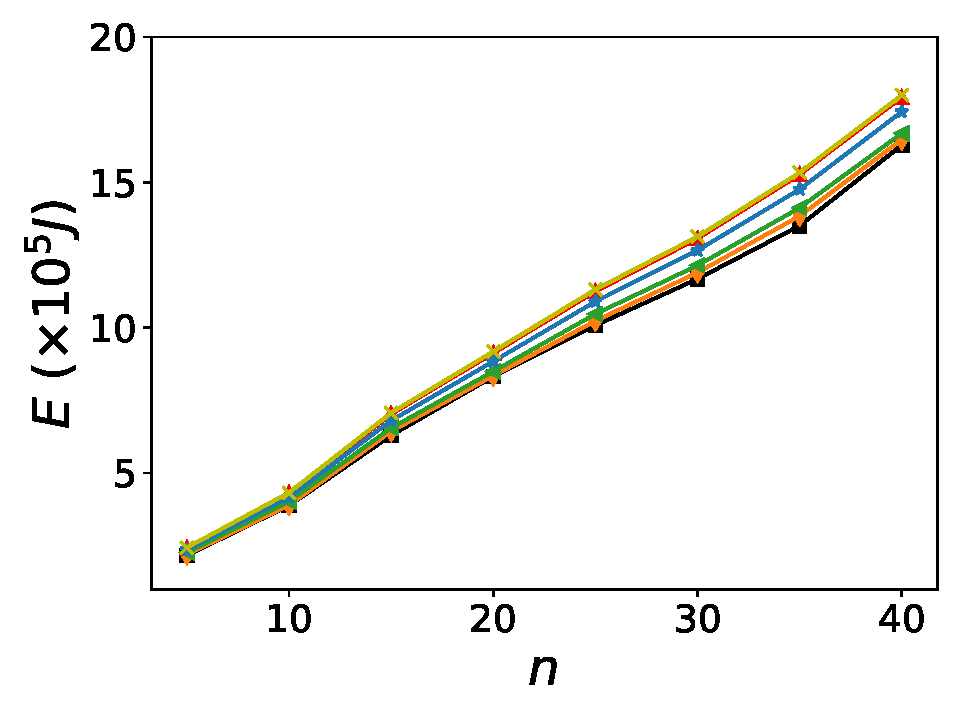
\includegraphics[width=.31\textwidth]{fig/exp_number_40.pdf}
			\label{subfig:number}
		}
		\hfill
		\subfloat[\footnotesize{The upper bound of coefficient of required time for data collection.}]{
			\centering
			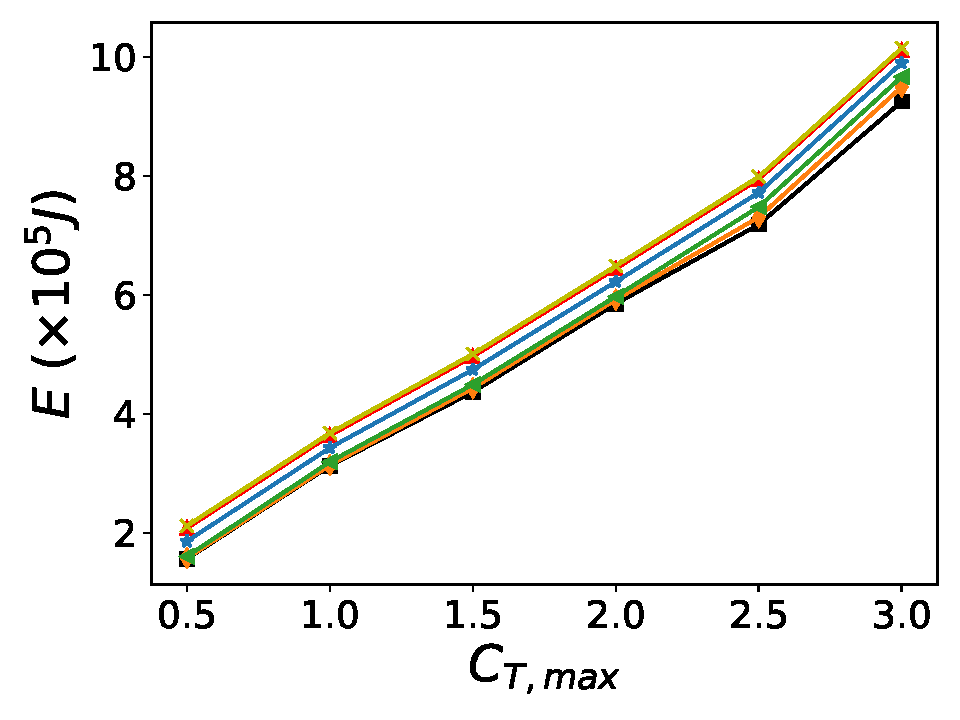
\includegraphics[width=.31\textwidth]{fig/exp_time.pdf}
			\label{subfig:time}
		}
		\hfill
		\subfloat[\footnotesize{The upper bound of height coefficient.}]{
			\centering
			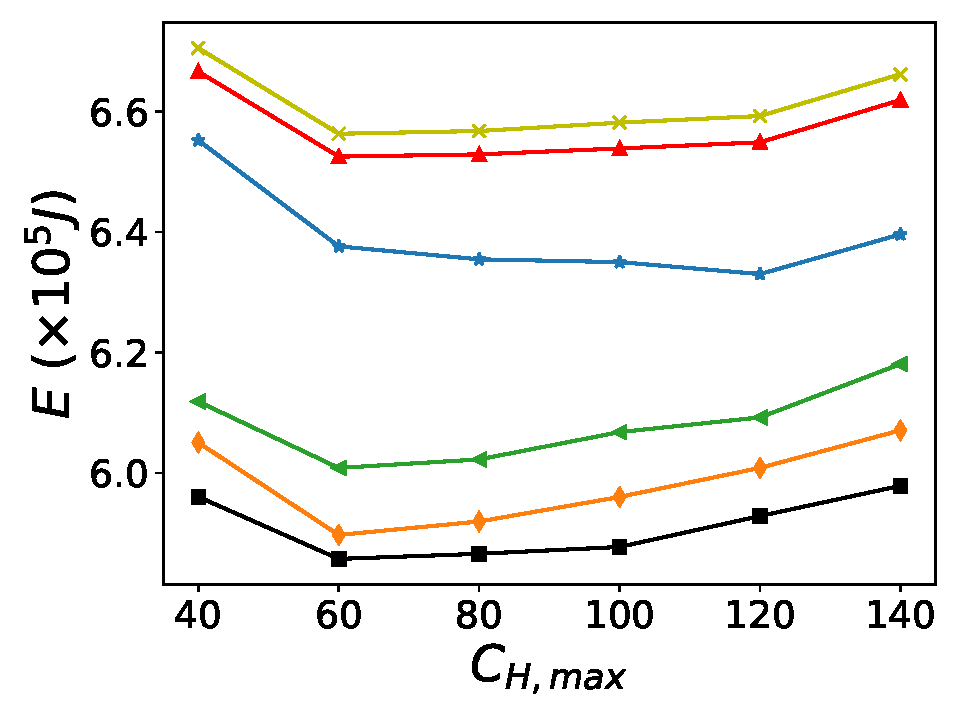
\includegraphics[width=.31\textwidth]{fig/exp_height.pdf}
			\label{subfig:height}
		}
		\hfill
		\subfloat[\footnotesize{The upper bound of width coefficient.}]{
			\centering
			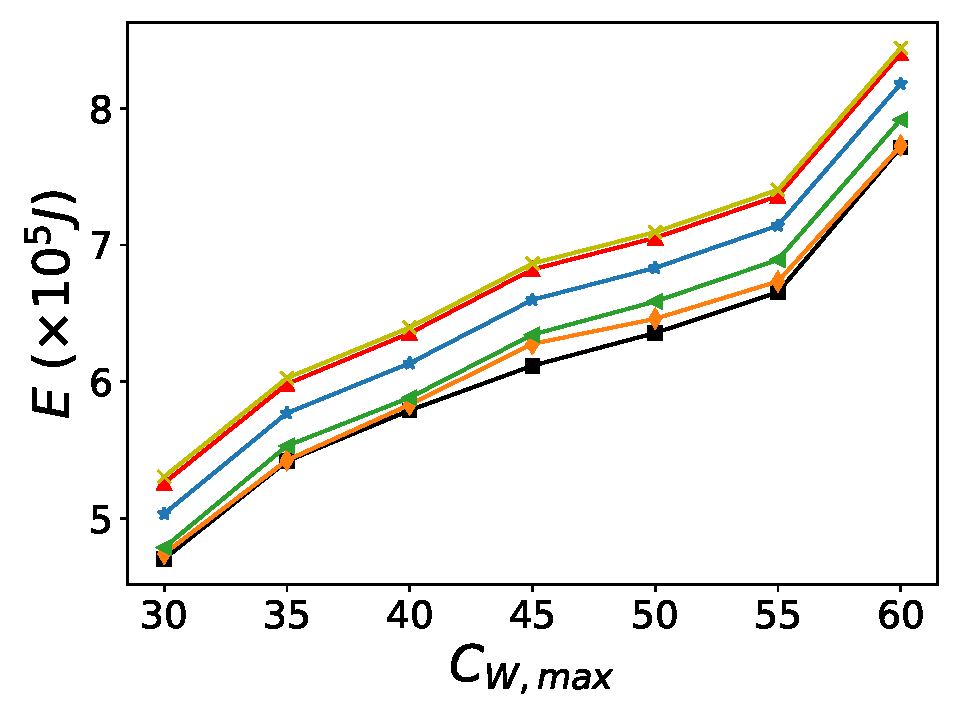
\includegraphics[width=.31\textwidth]{fig/exp_width.pdf}
			\label{subfig:width}
		}
		\hfill
		\subfloat[\footnotesize{The upper bound of swell coefficient of data transmission range.}]{
			\centering
			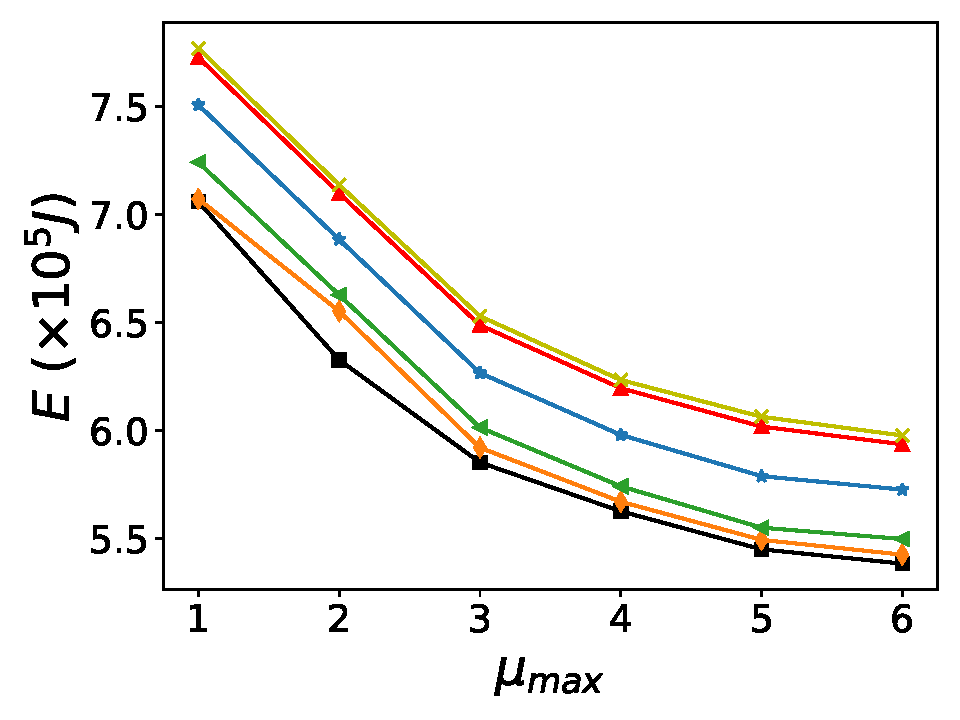
\includegraphics[width=.31\textwidth]{fig/exp_swell.pdf}
			\label{subfig:swell}
		}
		\hfill
		\subfloat[\footnotesize{The finest granularity of altitude change for UAV.}]{
			\centering
			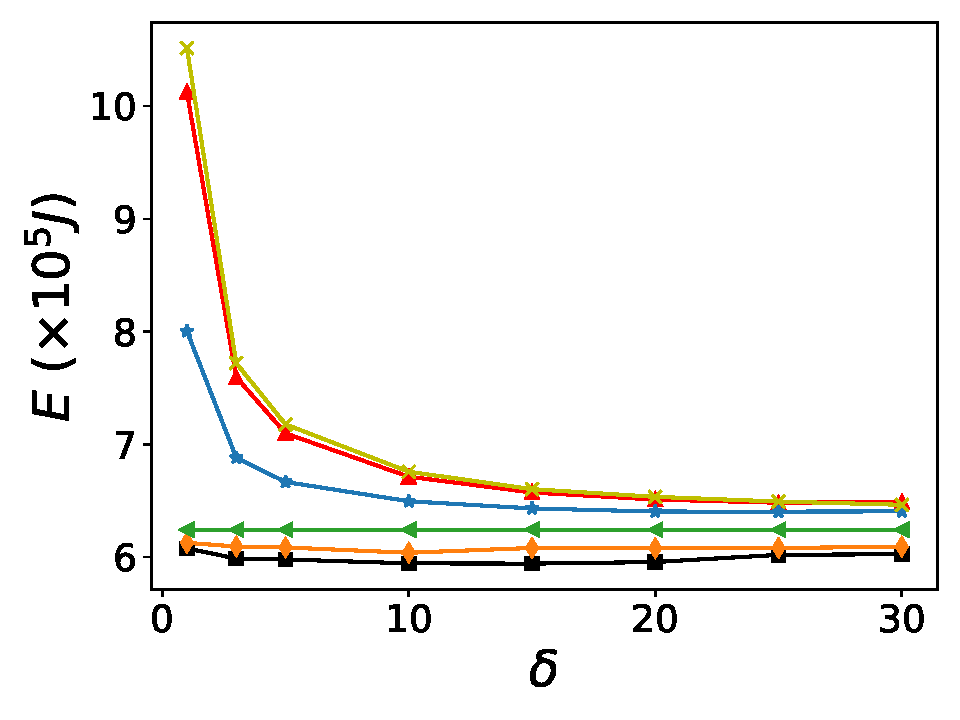
\includegraphics[width=.31\textwidth]{fig/exp_gran.pdf}
			\label{subfig:gran}
		}
		\hfill
		\subfloat[\footnotesize{The vertical consumption coefficient.}]{
			\centering
			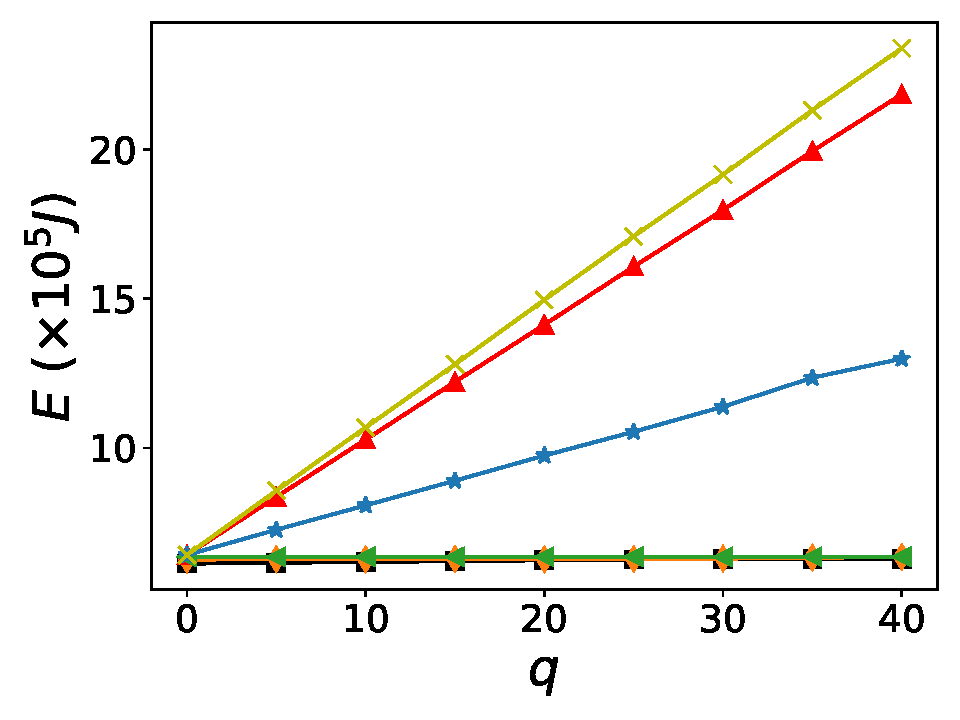
\includegraphics[width=.31\textwidth]{fig/exp_vertical.pdf}
			\label{subfig:vertical}
		}
		\hfill
		\subfloat[
			\footnotesize{The radius ratio of the control communication range to the data transmission range of a sensor.}
		]{
			\centering
			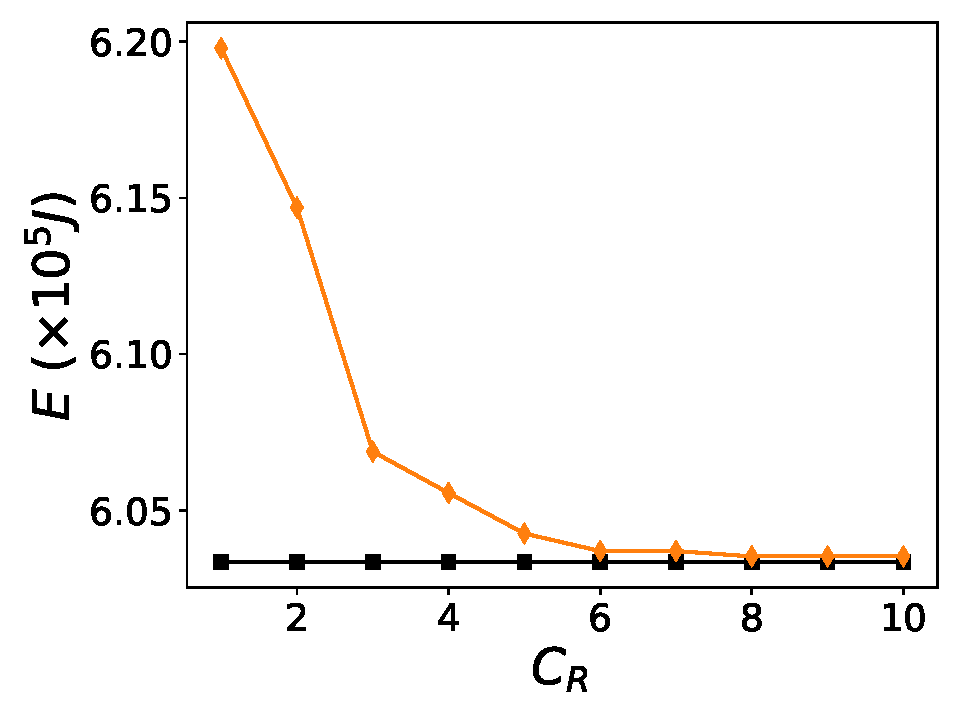
\includegraphics[width=.31\textwidth]{fig/exp_online.pdf}
			\label{subfig:online}
		}
		\hspace{.05\textwidth}
		\captionsetup[subfloat]{labelformat=empty} % 临时取消子图编号
		\subfloat[]{
			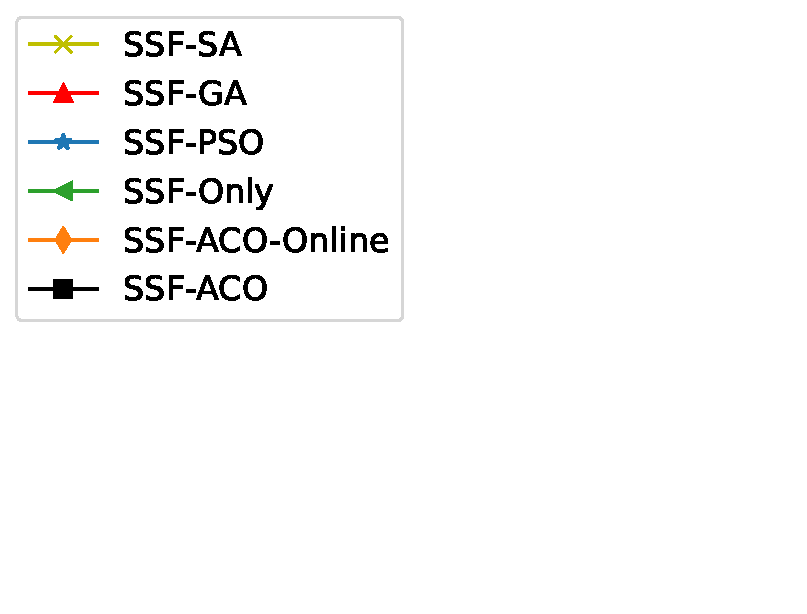
\includegraphics[width=.28\textwidth]{fig/legend.pdf}
		}
		\captionsetup[subfloat]{labelformat=parens} % 恢复子图编号
		\caption{Algorithm performance comparisons in UAV energy consumption.}
		\label{fig:exps}
	\end{figure*}
\end{revresponse}

\begin{revcomment}
	The dynamic nature of the sensor is not considered, such as movement, inaccurate position, failure and other problems.
\end{revcomment}
\begin{revresponse}
	We appreciate the reviewer's comment on the dynamics of sensors, which highlights important aspects that could influence the effectiveness the UAV scheduling.
	In the following, we will discuss the ground nodes (GNs) mobility, inaccurate position, failures, and unstable communication environment.

	\textbf{GN mobility.}
	GN mobility is an important factor in various UAV-assisted systems.
	However, our current work focuses on data collection from stationary sensors.
	In the scenarios we consider, the sensors are fixed in the environment to monitor infrastructures or natural conditions.
	Admittedly, a number of existing studies~\cite{GNmob1, GNmob2, GNmob3, GNmob4} have investigated GN mobility. %, primarily in the context of UAV-assisted task offloading or crowd sensing.
	In these studies, GNs typically refer to mobile user devices with significant movement, such as user-carried devices~\cite{GNmob1,GNmob2} or vehicles~\cite{GNmob3,GNmob4}, which are fundamentally different from the stationary GNs considered in our work.

	\textbf{Inaccurate position.}
	The proposed algorithm relies on the precise sensor positions.
	However, the inaccurate sensor localization leads to discrepancies between the UAV scheduling and actual environment.
	In our future, we intend to employ more advanced relative positioning techniques to reduce localization inaccuracy and incorporate error-tolerant strategies to improve the system's robustness and reliability.

	\textbf{Failures.}
	Failures may occur either before or during data transmission.
	Failures before transmission will result in the sensor being undetectable by the UAV.
	On the other hand, failures during the transmission process will lead to a disruption in the connection between the UAV and the sensor.
	The UAV will attemp to reconnect and, after reaching the maximum number of reconnection attempts, will abandon the connection.
	Regardless of whether reconnection is successful, the scheduling will be re-planned to ensure energy efficiency.
	% todo 在论文online那节加一段描述

	\textbf{Unstable communication environment.}
	The changes in the communication environment may lead to fluctuations in the transmission rate.
	When the UAV first detects the sensor, it will receive the sensor's guaranteed minimum transmission rate included the sensor's `ACK' message.
	When the guaranteed transmission rate is not met, the UAV's speed and altitude scheduling will be re-planned by our algorithm to adapt to the environment changes. 

\end{revresponse}

\begin{revcomment}
	Some minor suggestions:\\
	(1) The the first sentence in subsection 2.1, ``UAV'' → ``UAVs''.\\
	(2) Second paragraph of subsection 2.1, ``maintaining'' → ``maintained''.\\
	(3) Second paragraph of subsection 2.2, ``maintaining'' → ``and maintain''.\\
	(4) The ``='' in table 1.\\
	(5) Add $k \neq k'$ to equation (11), and $i \neq i'$ to equation (12).\\
	(6) The parameter $\mathbb{S}$ of algorithm 1 and 2 is neither used nor updated.\\
	(7) Line 2 of Algorithm 3, why set 20 to $Z$?
\end{revcomment}
\begin{revresponse}
	% todo 要不要把对应部分复制过来
	Thanks for your detailed suggestions.
	In response, we have made the following revisions.

	For points (1) to (4), we have improved the phrasing and table in the manuscript to mamke it more consistent and easier to read.

	For point (5), we would like to clarify that in Definition 1 in the manuscript, the condition $k<k'$ is defined. Additionally, in Equation (11), the condition $b_k < b_{k'}$ already implicitly ensures that $k\neq k'$.
	As for Equation (12), we have removed it along with its related content to improve the overall structure and clarity of the manuscript.

	For point (6), $\mathbb{S}$ is defined as a data structure that encapsulates essential sensor information. To improve clarity and facilitate readers' understanding, we have revised the manuscript by relocating the description of $\mathbb{S}$ closer to Algorithm 1 and 2.
	\begin{changes}
		For details, Alg. 1 takes the necessary sensor information as input and returns the optimal horizontal energy consumption.
		For simplicity, we denote these pieces of sensor information (such as $l_i$ and $r_i$) by $\mathbb{S}$.
	\end{changes}

	For point (7), we have added an explanation in the revised manuscript.
	\begin{changes}
		Here, $Z$ is set to 20 to balance solution quality and computational efficiency.
	\end{changes}
\end{revresponse}

\printpartbibliography{vertical-assumption,mgh,GNmob1,GNmob2,GNmob3,GNmob4}
